\section{Extended inference study: workload diversity, repetition and queueing}
\label{sec:extended-inference}

This study extends the initial five-second CPLA comparison to six recorded scenarios and 72 independently initialized service passes. Its purpose is to measure the behavior of the complete persistent inference services under repeated causal input, rather than infer deployment performance from parameter counts or a model-only forward pass. Both implementations retain their published weights. No TTC labels are read and no model is retrained. The experiment concerns inference on EvTTC and does not change the eAP accuracy results.

\subsection{Questions and prospective design}

The study asks four separate questions. First, does the response distribution reproduce across fresh processes and different scenes? Second, can each service deliver every update offered at 50\,Hz with a small bounded queue? Third, when buffering prevents an immediate history gap, does outstanding work remain bounded or accumulate into delayed responses? Fourth, do the optimized service outputs agree with independent native inference on the same causal observations? These questions require different statistics: a p95 over surviving outputs alone cannot answer the coverage or stability questions.

The campaign fixes the scenarios, interval-selection rule, repetitions, queue capacities, precision, rest policy and order before timing. It makes four passes per model and scenario with a two-packet queue, followed by two passes with a 64-packet queue. Each repetition alternates the first model in the pair, and the scenario order rotates. Thus each model occupies first position equally often within each queue policy. Every attempt is retained, including initialization failures, acquisition errors, dropped packets and subsequent refusals. The larger queue is a diagnostic of buffering and backlog; it does not establish an acceptable deployment latency.

\subsection{Sensor support and cohort selection}

All 32 physical sequences in the preserved transfer manifest are inspected using event-clock endpoints and causal annotation availability. A fixed 20\,ms grid begins at 700\,ms, or at the first event plus 620\,ms when that is later. The scout records every accepted and rejected slot. It does not inspect TTC, depth, velocity, RGB pixels, model predictions or measured latency when selecting the workload. The complete scout is reconstructed and checked before the campaign is frozen.

Six scenarios are declared to include cars and pedestrians, straight and lateral motion, different road configurations and different speed categories. For each, the longest uninterrupted accepted interval is selected; ties use the earliest interval. Invalid annotation slots are not removed and joined across a gap. The resulting intervals are listed in Table~\ref{tab:extended-cohorts}. This is an input-availability selection rule, not an unbiased random sample of all driving time: scenes and instants without a usable annotated target are outside the timed cohort.

\begin{table}[H]
\centering\footnotesize
\caption{\textbf{Distinct continuous sensor intervals.} Duration is the number of scheduled updates divided by 50; the last anchor is one period before the interval end. The same interval is replayed in each repetition.}
\label{tab:extended-cohorts}
\begin{tabular}{llrrr}
\toprule
ID & Sequence & Start (s) & Updates & Duration (s) \\
\midrule
S1 & CPLA-low & 16.76 & 370 & 7.40 \\
S2 & CCRm-medium-0-overlap-0 & 8.76 & 465 & 9.30 \\
S3 & CCRs-3-low-100-overlap-100 & 6.52 & 452 & 9.04 \\
S4 & CCRs-side-high & 11.98 & 260 & 5.20 \\
S5 & CPNA-high & 19.62 & 155 & 3.10 \\
S6 & CPNAO-high & 13.02 & 277 & 5.54 \\
\bottomrule
\end{tabular}

\end{table}

The longest usable interval is 465 updates, or 9.3\,s. Repeating this interval increases the evidence about run-to-run variation but does not create a longer unique recording. The six scenes are not joined into one synthetic continuous stream, and the experiment does not claim a 60-second uninterrupted sensor test. Each pass resets its process, history and caches and then consumes the complete registered interval.

\begin{table}[H]
\centering\small
\caption{\textbf{Observed RAW workload.} Counts come from the feeder in the first PHASE small-queue pass, including acquired packets later dropped by the consumer queue. Event rate is averaged over the offered interval; the preload archive also contains initialization history and RGB frames.}
\begin{tabular}{lrrrr}
\toprule
Scene & RAW packets & Events (M) & M events/s & Archive MiB \\
\midrule
S1 & 370/370 & 74.94 & 10.13 & 2026 \\
S2 & 465/465 & 135.44 & 14.56 & 3017 \\
S3 & 452/452 & 121.67 & 13.46 & 2834 \\
S4 & 260/260 & 103.46 & 19.90 & 2185 \\
S5 & 155/155 & 73.21 & 23.62 & 1506 \\
S6 & 277/277 & 79.47 & 14.35 & 1889 \\
\bottomrule
\end{tabular}

\end{table}

\subsection{Hardware, initialization and controlled execution choices}

Both services execute on the same NVIDIA RTX 5070 Ti Laptop GPU with 12\,GiB VRAM, on an AMD Ryzen 9 9955HX host with 32\,GiB system memory. The measured environment uses Python 3.11.15, PyTorch 2.11.0 with CUDA 12.8, and driver 591.86. Inference is FP32 with TF32 disabled. Both use two PyTorch CPU threads; PHASE additionally retains its eight RGB preparation workers. Garl uses one inter-op thread. The recorded configurations, rather than nominal hardware specifications alone, define the execution comparison.

Model loading, private RAW preload, the initial 600\,ms event history, synthetic shape priming, graph capture and feeder warmup precede measured arrivals. A fixed 15-second rest follows feeder warmup in both services. Host and GPU state are recorded around this rest, outside the measurement interval. The rest is a reproducible waiting policy, not proof of thermal equilibrium. Desktop scheduling and other host activity remain uncontrolled, and there is no attribution of a slow pass to temperature or a particular background process without direct evidence.

All timed passes finish before any native-reference GPU work begins. This removes the specific interleaving of full-decoder reference inference and subsequent timing present in the initial experiment. It does not equalize the architectures' own initialization costs or eliminate all device-state variation. Startup timings and memory envelopes are retained separately. No concurrent GPU experiment is launched by this campaign.

\begin{table}[H]
\centering\small
\caption{\textbf{Observed GPU state after the pre-stream rest.} Ranges are point-in-time observations across attempts, not continuous telemetry or temperature control. They do not identify the cause of an individual delay.}
\begin{tabular}{llrrr}
\toprule
Policy & Model & GPU temperature $^\circ$C & SM MHz & Power W \\
\midrule
bounded & PHASE & 62.0--74.0 & 210.0--1530.0 & 9.1--26.3 \\
bounded & Garl & 62.0--71.0 & 270.0--307.0 & 9.3--11.1 \\
buffered & PHASE & 62.0--65.0 & 255.0--307.0 & 9.4--10.1 \\
buffered & Garl & 63.0--66.0 & 255.0--292.0 & 9.6--10.1 \\
\bottomrule
\end{tabular}

\end{table}

\subsection{Complete persistent pipelines and architectural comparison}

PHASE executes its complete nine-component system: four modality-specific motion producers, two pair heads, two temporal context refiners and the residual fusion head. Its distributed system contains \LocalPhaseParameters{} parameters. The 1,955-parameter residual head is not substituted for the complete model when reporting size. Persistent event prefixes and exact reverse-transport summaries avoid rebuilding shared history, and native query graphs reduce dispatch overhead. RGB region preparation overlaps event execution, while an identity-checked cache reuses previously computed RGB producer features. Agreement of the resulting output chain with native inference is evaluated separately. Temporal readouts and final TTC predictions are recomputed.

Garl's TTC path uses paired RGB and event ResNet-50 backbones, feature fusion and a height-ratio TTC readout. The full checkpoint retains \LocalGarlStoredParameters{} stored parameters, including auxiliary foreground decoders. Those decoders are bypassed during TTC-only service because they do not contribute to the TTC output; they remain enabled in the independent native reference. The previously recorded execution profile counts \LocalGarlTTCParameters{} parameters in the TTC path, compared with \LocalPhaseExecutedParameters{} in called PHASE modules. These are module-execution parameter counts, not FLOPs or an exported pruned checkpoint size.

Garl receives the last two declared causal RGB endpoints and corresponding boxes in the common input contract. Event support is capped at 100\,ms per endpoint and uses the native 20-plane, first-event-relative representation. The actual endpoint interval is retained in the signed height-ratio conversion. Exact paired RGB backbone features may be reused; independent single-frame embeddings are not substituted for the native six-channel paired backbone. Event preparation may reuse unchanged endpoint tensors, but the event backbone, fusion and TTC heads execute on every completed request. Separate CUDA graphs cover the RGB and event/fusion branches. Neither service caches the final TTC output.

The services therefore have different computational structures despite receiving the same released observations. PHASE combines several compact motion and temporal modules and reuses shared history; Garl applies larger spatial backbones to paired sensor representations. Parameter count describes model storage and executed modules, while measured service time also includes ROI preparation, event encoding, memory movement, graph dispatch and synchronization. No FLOP estimate or asymptotic claim is substituted for measured response, and the results do not isolate a single architectural cause of a latency difference.

The local Garl implementation retains causal event packets in a deque and assembles an endpoint window only when required. On a representation-cache miss, its native-compatible CPU path masks the ROI, groups selected events by pixel and temporal plane using a stable sort, constructs the 20-plane time volume, and applies the released sampling convention before transfer to the GPU. PHASE instead advances its persistent event prefixes and queries the required representations on the GPU. These implementation choices are part of the measured pipelines. The results are not lower bounds on what a different numerically compatible Garl preprocessing implementation could achieve, and a long response cannot be attributed to backbone size alone.

The measured instrumentation also differs: Garl computes a prepared-sensor SHA-256 inside each completed call, while PHASE records causal metadata without hashing every prepared tensor. Both share the feeder's newly released frame checksums. This diagnostic overhead remains inside the reported service response; its isolated contribution is not measured or subtracted.

\subsection{Causality, input age and the measurement clock}

The feeder privately preloads RAW bytes, but releases each packet and newly available frame only at its scheduled causal query. Event conversion and copying, frame sealing, annotation validation, ROI preparation, CPU/GPU transfers, complete inference and host delivery remain within the response path. The initial history contains only observations preceding the first query. A supplied annotated region is assumed available at its declared sensor timestamp; object detection and tracking are not measured.

For scheduled arrival $a_i$, completed RAW availability $v_i$, consumer start $s_i$ and host TTC completion $c_i$, the recorded clocks are
\[
 R_i=c_i-a_i,\qquad A_i=c_i-v_i,\qquad S_i=c_i-s_i,
 \qquad Q_i=s_i-v_i.
\]
The primary response $R_i$ includes release lateness, acquisition and queueing. $S_i$ is service time and $Q_i$ is waiting after the payload is available. Subtracting acquisition or queueing would answer a different question. A 50\,Hz input has a 20\,ms period; response latency may exceed one period while throughput remains 50\,Hz if acquisition and service overlap. Conversely, a short model forward does not establish that the whole service keeps up.

Repeated RGB endpoints retain their original timestamps. Reuse is not presented as a new camera observation at every query. Garl's endpoint identities, source age, prepared-input hashes and cache decisions are recorded for each delivered output. PHASE records the causal event windows, RGB observations, geometry and temporal support used by its full prediction chain. The two systems can aggregate their released history differently; equal arrival packets do not imply identical internal representations.

PHASE's event windows end at the current query and can incorporate new events between RGB arrivals. Garl's native-compatible event volumes end at its declared RGB endpoints, so repeated calls can reuse the same underlying pair. Fifty requested outputs per second therefore does not mean fifty distinct RGB observations or independent predictions per second.

\begin{table}[H]
\centering\small
\caption{\textbf{Age of Garl's latest declared RGB endpoint.} Statistics use the independent native reference at every valid anchor, including anchors for which a timed service did not return a TTC. RGB pairs count distinct endpoint identities.}
\begin{tabular}{lrrrr}
\toprule
Scene & Native references & Age range ms & Median ms & RGB pairs \\
\midrule
S1 & 370/370 & 9.18--49.34 & 29.26 & 148 \\
S2 & 465/465 & 9.54--49.76 & 29.65 & 186 \\
S3 & 452/452 & 9.59--49.82 & 29.70 & 181 \\
S4 & 260/260 & 2.83--47.91 & 25.37 & 104 \\
S5 & 155/155 & 7.43--47.62 & 27.51 & 62 \\
S6 & 277/277 & 9.47--49.59 & 29.53 & 111 \\
\bottomrule
\end{tabular}

\end{table}

\subsection{Independent native verification and evidence preservation}

After all 72 timing attempts, each scenario is reread from disk by an independent native reference for each model. The reference is computed once per unique anchor and then compared with every delivered output from every repetition. This avoids repeatedly heating the GPU with the reference between timed passes while still checking all measured predictions. It does not turn repeated timings into independent prediction samples.

For Garl, verification reconstructs full-frame RGB normalization and native event representations, checks the prepared sensor tensor's SHA-256, and compares both raw heights and signed TTC with relative and absolute tolerances of $10^{-5}$. The unmodified native model executes its auxiliary decoders. For PHASE, verification uses the original uncached predictor, checks all three TTC components with its preserved tolerance contract, and compares causal input metadata exactly. PHASE's metadata receipt is not a hash of every prepared tensor or RAW byte; source-stat, annotation and model/source checks supplement numerical parity. That distinction remains explicit.

The model sources, historical service overlay, model inventories, manifests, timed launchers and measurement commands are frozen before timing. The independent native-reference implementation is included in that freeze. Integrity is checked after timing and around native-reference computation, then checked again before evidence archival. Publication regenerates the numerical comparisons from the saved reference and measured prediction records, verifies file hashes, and rejects altered evidence or missing declared attempts. Numerical disagreements are retained as failed checks; they are not converted into successful native validation. Failed reference computations and absent service predictions remain distinct from successful numerical agreement.

A later-added controller waits for the timed campaign to close and invokes the frozen native-reference implementation. Its job list and executed source are recorded after timing; the controller itself was not prospectively frozen in this campaign. The publication sealer is also a later analysis tool. These stages do not alter the measured services or the frozen native-reference arithmetic.

The recorded Git identifier denotes the base checkout. Exact file digests and archived source snapshots identify the executed revision, including the new benchmark launchers; the base commit alone is not presented as containing those new files. The final publication also preserves the byte identity of the archiver actually executed and its supplemental evidence-sealing script.

\subsection{Numerical agreement and admission of performance claims}

The independent references exposed numerical differences beyond the frozen tolerance in some delivered PHASE outputs. The analysis therefore distinguishes complete delivery from admission under the full numerical contract. An admitted run must deliver every scheduled output and pass all required native checks, including intermediate TTC components. A run that delivers every output but fails an intermediate check remains a complete delivery; its full-service p95 is withheld from admitted comparisons. The tolerance and the measured service code are unchanged.

This reporting distinction was made explicit after inspecting the first numerical failures. It is a retrospective accounting clarification, not a changed timing protocol or a relaxed acceptance threshold. The per-pass timing tables retain the measured response distributions, including numerically rejected outputs, with a separate failed-parity count. The aggregate deadline counts likewise describe delivered timing, not the number of fully validated timely predictions.

The frozen PHASE numerical contract uses relative and absolute tolerances of $10^{-5}$ for each of its three TTC outputs. These differences measure agreement with native inference, not error against TTC labels.

For the fused output, 0 of 4,720 delivered comparisons exceed the contract, covering 0 distinct scene/anchor pairs.

For the event output, 0 of 4,720 delivered comparisons exceed the contract, covering 0 distinct scene/anchor pairs.

For the rgb output, 6 of 4,720 delivered comparisons exceed the contract, covering 3 distinct scene/anchor pairs.


\begin{table}[H]
\centering\footnotesize
\caption{\textbf{PHASE component agreement with native inference.} Checks and failures count repeated delivered comparisons; anchors count distinct failed anchors within each scene, and runs count affected repetitions. Maximum errors use all delivered comparisons. Complete delivery alone does not establish numerical admission.}
\begin{tabular}{llrrrrrr}
\toprule
Scene & Output & Checks & Failures & Anchors & Runs & Max abs. s & Max rel. \\
\midrule
S1 & Fused & 993 & 0 & 0 & 0 & 8.11e-06 & 1.74e-06 \\
S1 & Event & 993 & 0 & 0 & 0 & 0.00e+00 & 0.00e+00 \\
S1 & RGB & 993 & 0 & 0 & 0 & 1.34e-05 & 2.68e-06 \\
S2 & Fused & 942 & 0 & 0 & 0 & 3.59e-04 & 7.17e-06 \\
S2 & Event & 942 & 0 & 0 & 0 & 0.00e+00 & 0.00e+00 \\
S2 & RGB & 942 & 6 & 3 & 2 & 1.22e-03 & 2.11e-05 \\
S3 & Fused & 1365 & 0 & 0 & 0 & 4.29e-06 & 6.95e-07 \\
S3 & Event & 1365 & 0 & 0 & 0 & 0.00e+00 & 0.00e+00 \\
S3 & RGB & 1365 & 0 & 0 & 0 & 8.58e-06 & 1.14e-06 \\
S4 & Fused & 532 & 0 & 0 & 0 & 4.29e-06 & 9.52e-07 \\
S4 & Event & 532 & 0 & 0 & 0 & 0.00e+00 & 0.00e+00 \\
S4 & RGB & 532 & 0 & 0 & 0 & 6.68e-06 & 1.43e-06 \\
S5 & Fused & 322 & 0 & 0 & 0 & 6.68e-06 & 1.32e-06 \\
S5 & Event & 322 & 0 & 0 & 0 & 0.00e+00 & 0.00e+00 \\
S5 & RGB & 322 & 0 & 0 & 0 & 1.62e-05 & 2.39e-06 \\
S6 & Fused & 566 & 0 & 0 & 0 & 1.07e-04 & 3.24e-06 \\
S6 & Event & 566 & 0 & 0 & 0 & 0.00e+00 & 0.00e+00 \\
S6 & RGB & 566 & 0 & 0 & 0 & 5.91e-05 & 3.28e-06 \\
\bottomrule
\end{tabular}

\end{table}

\subsection{Small-queue service response across scenarios}

\begin{table}[H]
\centering\small
\caption{\textbf{Primary 50\,Hz service with queue capacity two.} Four repetitions per model and scene. Delivered runs return every offered update; admitted runs additionally pass every native numerical check. Median p95 and its range are reported only when all four runs are admitted; a dash is not zero latency.}
\label{tab:extended-bounded}
\begin{tabular}{llrrrrr}
\toprule
Scene & Model & Delivered & Admitted & Outputs & p95 & p95 range \\
\midrule
S1 & PHASE & 0/4 & 0/4 & 253/1480 & --- & --- \\
S1 & Garl & 0/4 & 0/4 & 12/1480 & --- & --- \\
S2 & PHASE & 0/4 & 0/4 & 12/1860 & --- & --- \\
S2 & Garl & 0/4 & 0/4 & 12/1860 & --- & --- \\
S3 & PHASE & 1/4 & 1/4 & 461/1808 & --- & --- \\
S3 & Garl & 0/4 & 0/4 & 12/1808 & --- & --- \\
S4 & PHASE & 0/4 & 0/4 & 12/1040 & --- & --- \\
S4 & Garl & 0/4 & 0/4 & 12/1040 & --- & --- \\
S5 & PHASE & 0/4 & 0/4 & 12/620 & --- & --- \\
S5 & Garl & 0/4 & 0/4 & 12/620 & --- & --- \\
S6 & PHASE & 0/4 & 0/4 & 12/1108 & --- & --- \\
S6 & Garl & 0/4 & 0/4 & 12/1108 & --- & --- \\
\bottomrule
\end{tabular}

\end{table}

\begin{figure}[H]
\centering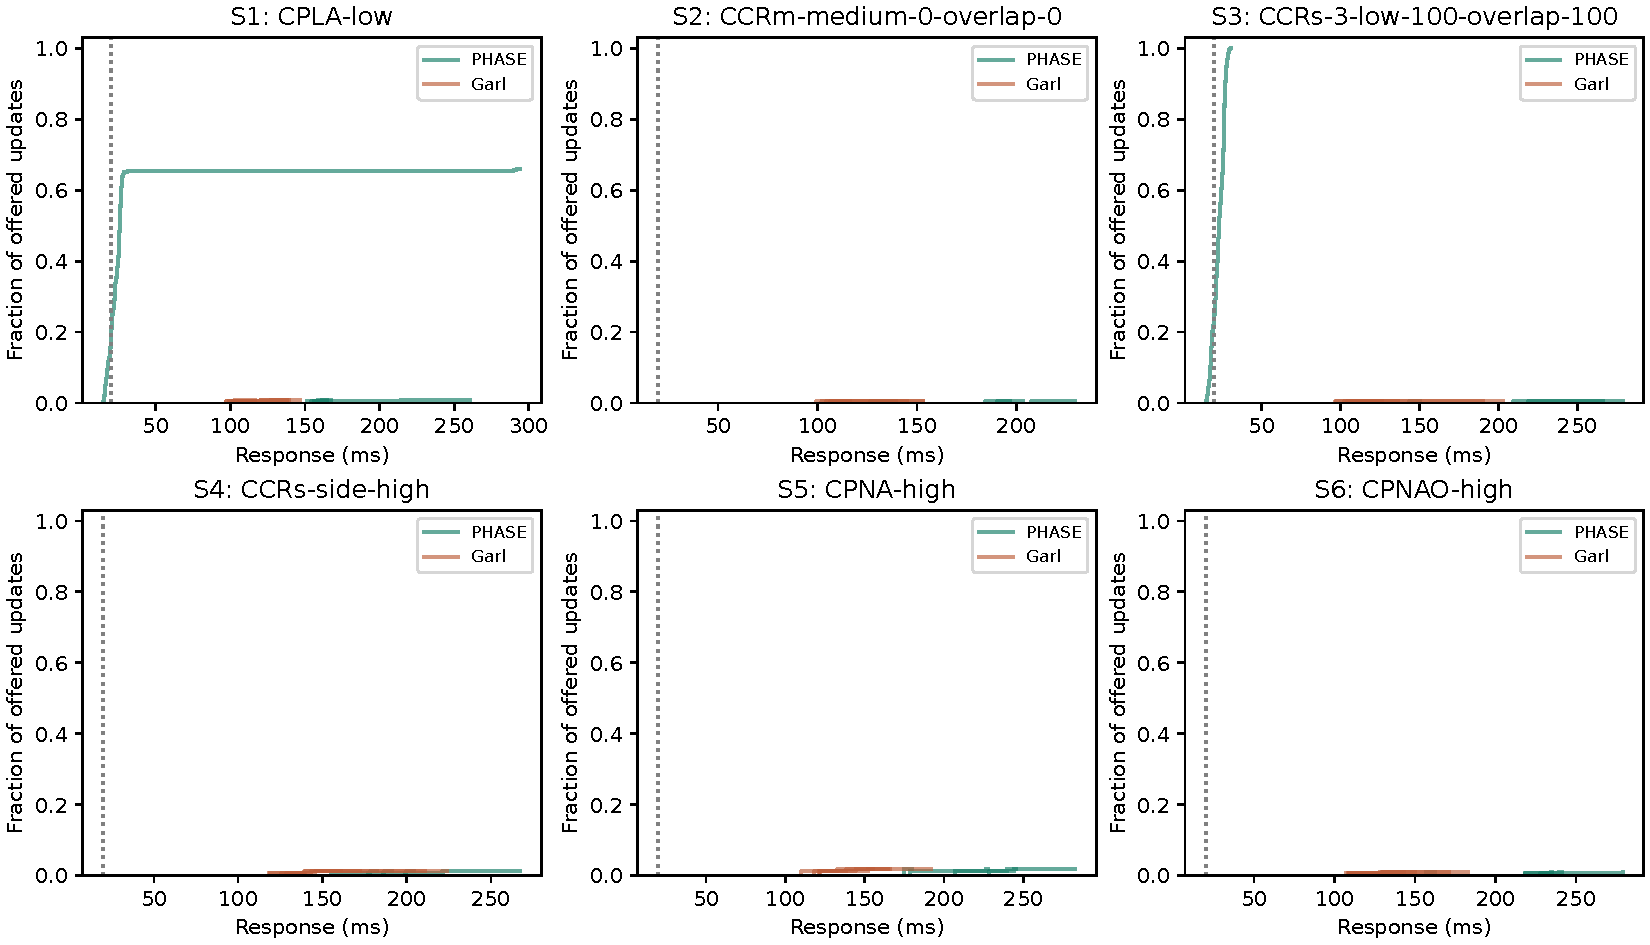
\includegraphics[width=\linewidth]{figures/extended_coverage_cdf.pdf}
\caption{\textbf{Response and coverage in the primary experiment.} Each curve is one attempted replay, with all offered updates in the denominator. Curves that stop below one indicate missing outputs. The dotted line marks 20\,ms.}
\end{figure}

With the two-packet queue, PHASE completed 1/24 full replays and delivered 762/7,916 outputs (9.6\%). Of all offered updates, 178 (2.2\%) completed below 20\,ms. Strict native parity admitted 1/24 full replays; 0 delivered outputs failed at least one required numerical check.

With the two-packet queue, Garl completed 0/24 full replays and delivered 72/7,916 outputs (0.9\%). Of all offered updates, 0 (0.0\%) completed below 20\,ms. Strict native parity admitted 0/24 full replays; 0 delivered outputs failed at least one required numerical check.

With the 64-packet queue, PHASE completed 12/12 full replays and delivered 3,958/3,958 outputs (100.0\%). Of all offered updates, 1,217 (30.7\%) completed below 20\,ms. Strict native parity admitted 10/12 full replays; 6 delivered outputs failed at least one required numerical check.

With the 64-packet queue, Garl completed 7/12 full replays and delivered 3,816/3,958 outputs (96.4\%). Of all offered updates, 429 (10.8\%) completed below 20\,ms. Strict native parity admitted 7/12 full replays; 0 delivered outputs failed at least one required numerical check.


\subsection{Buffering, outstanding work and throughput}

\begin{table}[H]
\centering\small
\caption{\textbf{Buffered diagnostic with queue capacity 64.} Two repetitions per model and scene, retaining the same 50\,Hz input schedule. Full-population p95 includes any accumulated queue delay and requires both runs to be admitted. These measurements are separate from the small-queue primary experiment.}
\label{tab:extended-buffered}
\begin{tabular}{llrrrrr}
\toprule
Scene & Model & Delivered & Admitted & Outputs & p95 & p95 range \\
\midrule
S1 & PHASE & 2/2 & 2/2 & 740/740 & 121.66 & 101.55--141.77 \\
S1 & Garl & 2/2 & 2/2 & 740/740 & 2932.78 & 2850.89--3014.67 \\
S2 & PHASE & 2/2 & 0/2 & 930/930 & --- & --- \\
S2 & Garl & 2/2 & 2/2 & 930/930 & 1741.70 & 1736.81--1746.58 \\
S3 & PHASE & 2/2 & 2/2 & 904/904 & 105.15 & 102.06--108.25 \\
S3 & Garl & 0/2 & 0/2 & 897/904 & --- & --- \\
S4 & PHASE & 2/2 & 2/2 & 520/520 & 226.71 & 225.63--227.78 \\
S4 & Garl & 0/2 & 0/2 & 387/520 & --- & --- \\
S5 & PHASE & 2/2 & 2/2 & 310/310 & 175.53 & 164.74--186.33 \\
S5 & Garl & 2/2 & 2/2 & 310/310 & 4934.71 & 4894.39--4975.03 \\
S6 & PHASE & 2/2 & 2/2 & 554/554 & 103.72 & 94.87--112.56 \\
S6 & Garl & 1/2 & 1/2 & 552/554 & --- & --- \\
\bottomrule
\end{tabular}

\end{table}

\begin{figure}[H]
\centering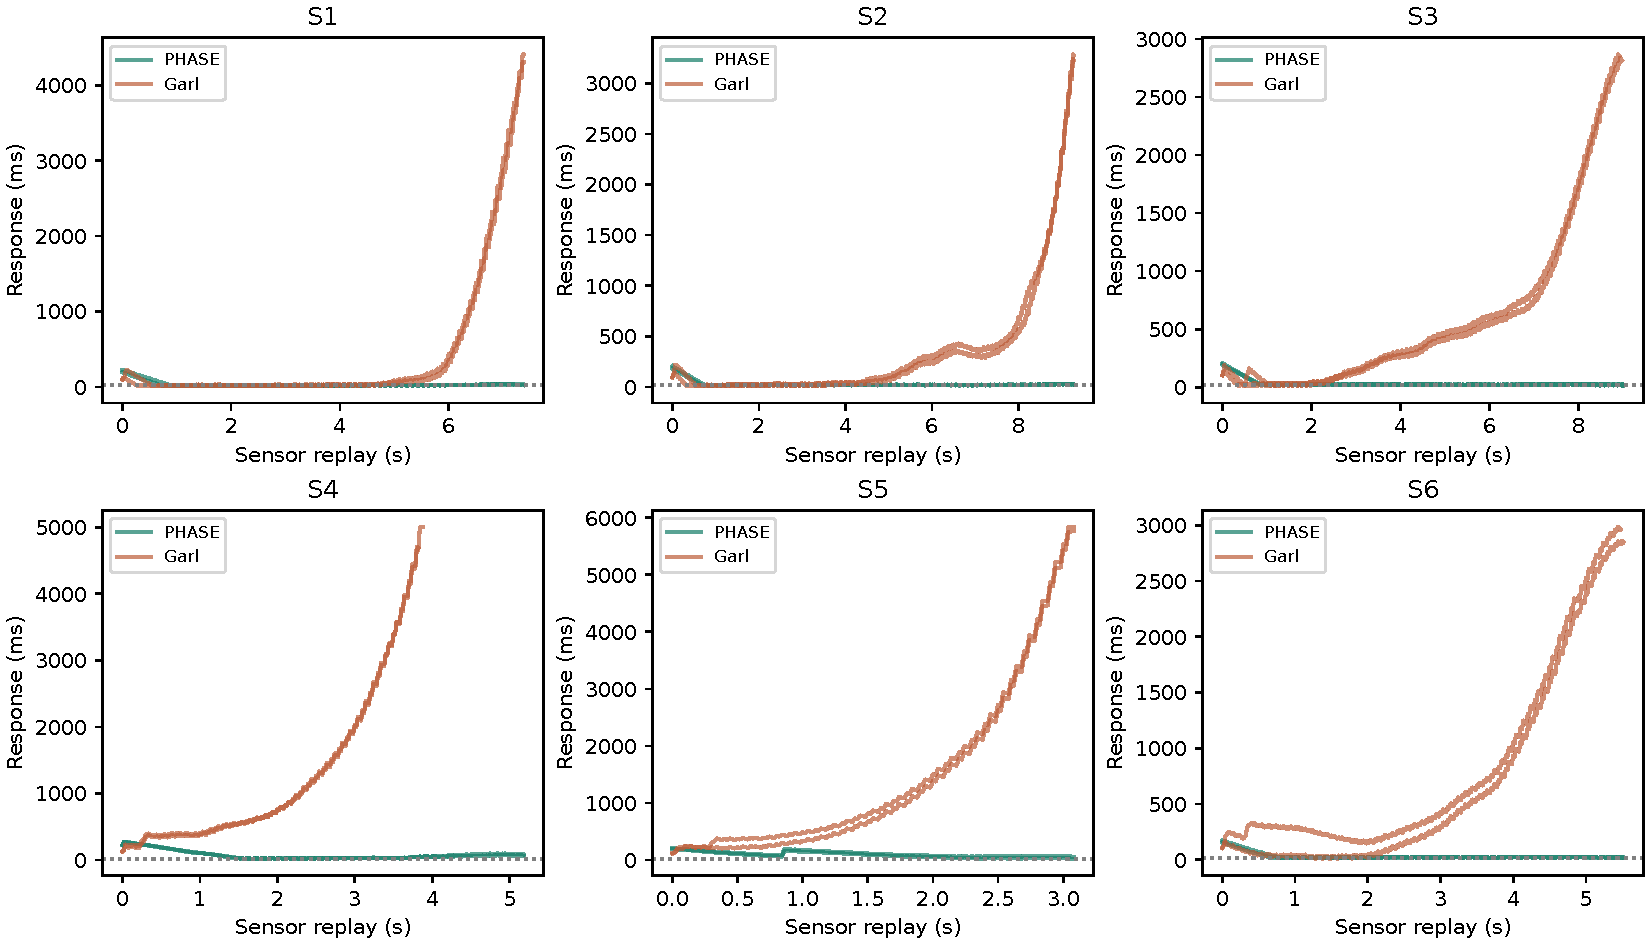
\includegraphics[width=\linewidth]{figures/extended_buffered_traces.pdf}
\caption{\textbf{Response traces with additional buffering.} A rising response trajectory indicates increasing delay relative to sensor time. Missing tails remain missing; no later prediction is invented to complete a curve.}
\end{figure}

The buffered diagnostic distinguishes short overload bursts from the immediate cascade caused by a dropped RAW packet. Both services require contiguous causal history. A missing packet invalidates that history and latches subsequent requests into refusal until a fresh replay; the campaign does not silently refill history, skip sensor time or emit stale TTC. The reported failed responses therefore include correlated refusals, not just independent numerical failures. Recovery behavior is documented rather than changed during this comparison.

Output rate is the number of successful deliveries divided by the interval from the first scheduled arrival to the last successful completion. For an incomplete run this is a diagnostic over its delivered prefix, not sustained capacity for the full offered recording. Drain time measures how far the last valid completion extends beyond the end of the offered interval. Neither quantity is calculated as $1000/\mathrm{p95}$, and neither alone establishes a real-time deadline guarantee. The 64-packet queue can reduce packet loss while allowing responses to become too old for an application.

\subsection{Initial response and later stream behavior}

Inspection of the first completed campaign round showed that an early long service call could fill the small queue and trigger the history-gap cascade. The following breakdown was therefore added retrospectively as a descriptive diagnostic; it is not a prospectively specified primary endpoint or a reason to remove the initial delay. It compares the first response, the p95 of the entire stream, and the p95 of the latter half of scheduled anchors. Each latency column is the median across the two buffered repetitions and is admitted only when both complete the entire interval with native parity. D/A/N gives complete deliveries, admitted runs and declared attempts. The latter half is fixed by anchor index, rather than selected for its measured speed.

\begin{table}[H]
\centering\small
\caption{\textbf{Retrospective initial/later response breakdown, in milliseconds.} Queue capacity 64. The later-window statistic retains its explicit subset definition and is not substituted for complete-stream latency or described as a guaranteed steady-state bound.}
\begin{tabular}{llrrrr}
\toprule
Scene & Model & D/A/N & First response & Full p95 & Latter-half p95 \\
\midrule
S1 & PHASE & 2/2/2 & 208.08 & 121.66 & 36.44 \\
S1 & Garl & 2/2/2 & 99.62 & 2932.78 & 3644.65 \\
S2 & PHASE & 2/0/2 & --- & --- & --- \\
S2 & Garl & 2/2/2 & 96.75 & 1741.70 & 2407.18 \\
S3 & PHASE & 2/2/2 & 199.66 & 105.15 & 27.54 \\
S3 & Garl & 0/0/2 & --- & --- & --- \\
S4 & PHASE & 2/2/2 & 223.12 & 226.71 & 81.17 \\
S4 & Garl & 0/0/2 & --- & --- & --- \\
S5 & PHASE & 2/2/2 & 200.88 & 175.53 & 89.66 \\
S5 & Garl & 2/2/2 & 115.68 & 4934.71 & 5484.29 \\
S6 & PHASE & 2/2/2 & 162.80 & 103.72 & 27.04 \\
S6 & Garl & 1/1/2 & --- & --- & --- \\
\bottomrule
\end{tabular}

\end{table}

\subsection{Memory, initialization and repeated-pass accounting}

\begin{table}[H]
\centering\small
\caption{\textbf{All attempts and service allocation.} CUDA peaks include resident model, persistent state, graph buffers and stream allocations after the counter reset. Values are allocated MiB, not the allocator's additional reserved capacity.}
\begin{tabular}{llrrrr}
\toprule
Queue policy & Model & Delivered & Admitted & Outputs & CUDA peak MiB \\
\midrule
bounded & PHASE & 1/24 & 1/24 & 762/7916 & 2969--2969 \\
bounded & Garl & 0/24 & 0/24 & 72/7916 & 966--966 \\
buffered & PHASE & 12/12 & 10/12 & 3958/3958 & 2969--2969 \\
buffered & Garl & 7/12 & 7/12 & 3816/3958 & 966--966 \\
\bottomrule
\end{tabular}

\end{table}

The RAW feeder declares a conservative 12\,GiB numeric memory envelope, accounting for preload, frame tokens, bounded payloads and scratch space. This is an upper bound rather than measured process RSS, and Python objects, HDF5 internals and output receipts are outside that numeric envelope. A larger queue changes this bound even when immutable frame tokens are shared. Complete startup receipts record RAW preload, model/service initialization, history preparation and graph setup separately from response latency.

\begin{table}[H]
\centering\footnotesize
\caption{\textbf{Initialization and reuse diagnostics.} Preload and model/priming columns give medians across the declared scenes and repetitions, in seconds. Model/priming excludes source audits, RAW history initialization and the fixed rest. Garl graph capture is recorded separately. Cache hits are conditional on attempted model updates, not new sensor frames; reserved MiB is the PyTorch allocator's peak reserve.}
\begin{tabular}{llrrrr}
\toprule
Policy & Model & Preload s & Model/prime s & RGB hits & Reserved MiB \\
\midrule
bounded & PHASE & 2.80 & 9.72 & 446/762 & 3428--3428 \\
bounded & Garl & 2.48 & 2.34 & 32/72 & 1110--1110 \\
buffered & PHASE & 2.61 & 9.91 & 2374/3958 & 3428--3428 \\
buffered & Garl & 2.52 & 2.38 & 2289/3816 & 1110--1110 \\
\bottomrule
\end{tabular}

\end{table}

The following tables retain each repetition instead of pooling correlated windows as if they were independent experiments. Per-pass p50, p95 and p99 are conditional on delivered outputs when coverage is incomplete; only the summary tables apply the all-repetitions full-coverage and native-parity admission rule. The Parity column counts delivered updates failing at least one required numerical check; it is separate from missing or refused outputs. Repetitions measure execution variability with fixed trained weights, not variation across training seeds. Six scenes are insufficient for a broad claim about all event-camera workloads, and no window-level confidence interval is used to imply that they are.

\begingroup\footnotesize
\begin{longtable}{llrrrrrrr}
\toprule
Pass & Model & Outputs & p50 & p95 & p99 & Drops & Failed & Parity \\
\midrule
\endhead
Q2 S1 R1 & PHASE & 244/370 & 23.03 & 27.29 & 178.29 & 12 & 114 & 0 \\
Q2 S1 R1 & Garl & 3/370 & 127.12 & 144.71 & 146.28 & 5 & 362 & 0 \\
Q2 S2 R1 & PHASE & 3/465 & 133.16 & 138.70 & 139.20 & 4 & 458 & 0 \\
Q2 S2 R1 & Garl & 3/465 & 129.27 & 150.50 & 152.39 & 5 & 457 & 0 \\
Q2 S3 R1 & PHASE & 452/452 & 23.03 & 27.84 & 29.25 & 0 & 0 & 0 \\
Q2 S3 R1 & Garl & 3/452 & 131.36 & 195.61 & 201.32 & 7 & 442 & 0 \\
Q2 S4 R1 & PHASE & 3/260 & 199.53 & 203.64 & 204.01 & 7 & 250 & 0 \\
Q2 S4 R1 & Garl & 3/260 & 145.48 & 204.50 & 209.75 & 8 & 249 & 0 \\
Q2 S5 R1 & PHASE & 3/155 & 239.72 & 278.52 & 281.97 & 12 & 140 & 0 \\
Q2 S5 R1 & Garl & 3/155 & 138.56 & 153.57 & 154.90 & 5 & 147 & 0 \\
Q2 S6 R1 & PHASE & 3/277 & 239.36 & 240.93 & 241.07 & 9 & 265 & 0 \\
Q2 S6 R1 & Garl & 3/277 & 127.94 & 177.18 & 181.56 & 7 & 267 & 0 \\
Q2 S2 R2 & Garl & 3/465 & 131.17 & 150.88 & 152.63 & 5 & 457 & 0 \\
Q2 S2 R2 & PHASE & 3/465 & 197.07 & 202.68 & 203.18 & 7 & 455 & 0 \\
Q2 S3 R2 & Garl & 3/452 & 119.24 & 134.44 & 135.79 & 4 & 445 & 0 \\
Q2 S3 R2 & PHASE & 3/452 & 264.56 & 266.23 & 266.37 & 11 & 438 & 0 \\
Q2 S4 R2 & Garl & 3/260 & 139.82 & 159.03 & 160.73 & 5 & 252 & 0 \\
Q2 S4 R2 & PHASE & 3/260 & 177.97 & 181.99 & 182.35 & 7 & 250 & 0 \\
Q2 S5 R2 & Garl & 3/155 & 132.92 & 161.83 & 164.40 & 5 & 147 & 0 \\
Q2 S5 R2 & PHASE & 3/155 & 226.56 & 227.51 & 227.59 & 9 & 143 & 0 \\
Q2 S6 R2 & Garl & 3/277 & 129.57 & 148.17 & 149.82 & 5 & 269 & 0 \\
Q2 S6 R2 & PHASE & 3/277 & 234.12 & 235.14 & 235.23 & 9 & 265 & 0 \\
Q2 S1 R2 & Garl & 3/370 & 119.98 & 136.10 & 137.53 & 4 & 363 & 0 \\
Q2 S1 R2 & PHASE & 3/370 & 213.91 & 255.96 & 259.70 & 10 & 357 & 0 \\
Q2 S3 R3 & PHASE & 3/452 & 278.24 & 278.80 & 278.85 & 11 & 438 & 0 \\
Q2 S3 R3 & Garl & 3/452 & 117.34 & 182.77 & 188.59 & 7 & 442 & 0 \\
Q2 S4 R3 & PHASE & 3/260 & 221.28 & 262.92 & 266.62 & 11 & 246 & 0 \\
Q2 S4 R3 & Garl & 3/260 & 139.17 & 215.36 & 222.13 & 9 & 248 & 0 \\
Q2 S5 R3 & PHASE & 3/155 & 174.80 & 179.38 & 179.79 & 6 & 146 & 0 \\
Q2 S5 R3 & Garl & 3/155 & 144.43 & 164.01 & 165.75 & 6 & 146 & 0 \\
Q2 S6 R3 & PHASE & 3/277 & 156.86 & 161.58 & 162.00 & 6 & 268 & 0 \\
Q2 S6 R3 & Garl & 3/277 & 129.98 & 166.71 & 169.97 & 6 & 268 & 0 \\
Q2 S1 R3 & PHASE & 3/370 & 160.98 & 166.50 & 166.99 & 5 & 362 & 0 \\
Q2 S1 R3 & Garl & 3/370 & 102.63 & 115.32 & 116.45 & 3 & 364 & 0 \\
Q2 S2 R3 & PHASE & 3/465 & 224.33 & 229.12 & 229.55 & 9 & 453 & 0 \\
Q2 S2 R3 & Garl & 3/465 & 102.28 & 114.94 & 116.07 & 3 & 459 & 0 \\
Q2 S4 R4 & Garl & 3/260 & 143.31 & 169.29 & 171.59 & 6 & 251 & 0 \\
Q2 S4 R4 & PHASE & 3/260 & 186.28 & 190.79 & 191.19 & 7 & 250 & 0 \\
Q2 S5 R4 & Garl & 3/155 & 152.29 & 188.11 & 191.29 & 7 & 145 & 0 \\
Q2 S5 R4 & PHASE & 3/155 & 244.38 & 245.06 & 245.12 & 10 & 142 & 0 \\
Q2 S6 R4 & Garl & 3/277 & 129.83 & 141.51 & 142.55 & 5 & 269 & 0 \\
Q2 S6 R4 & PHASE & 3/277 & 278.82 & 279.07 & 279.09 & 11 & 263 & 0 \\
Q2 S1 R4 & Garl & 3/370 & 119.94 & 137.35 & 138.89 & 4 & 363 & 0 \\
Q2 S1 R4 & PHASE & 3/370 & 158.25 & 163.81 & 164.30 & 5 & 362 & 0 \\
Q2 S2 R4 & Garl & 3/465 & 125.86 & 142.90 & 144.42 & 5 & 457 & 0 \\
Q2 S2 R4 & PHASE & 3/465 & 190.76 & 196.23 & 196.72 & 7 & 455 & 0 \\
Q2 S3 R4 & Garl & 3/452 & 124.17 & 126.28 & 126.47 & 4 & 445 & 0 \\
Q2 S3 R4 & PHASE & 3/452 & 144.26 & 149.57 & 150.04 & 5 & 444 & 0 \\
Q64 S1 R1 & PHASE & 370/370 & 22.90 & 101.55 & 173.70 & 0 & 0 & 0 \\
Q64 S1 R1 & Garl & 370/370 & 30.53 & 2850.89 & 4089.93 & 0 & 0 & 0 \\
Q64 S2 R1 & PHASE & 465/465 & 22.76 & 72.18 & 157.84 & 0 & 0 & 3 \\
Q64 S2 R1 & Garl & 465/465 & 64.37 & 1736.81 & 2967.25 & 0 & 0 & 0 \\
Q64 S3 R1 & PHASE & 452/452 & 22.52 & 108.25 & 184.94 & 0 & 0 & 0 \\
Q64 S3 R1 & Garl & 450/452 & 321.58 & 2407.23 & 2769.95 & 2 & 0 & 0 \\
Q64 S4 R1 & PHASE & 260/260 & 50.76 & 227.78 & 263.92 & 0 & 0 & 0 \\
Q64 S4 R1 & Garl & 195/260 & 697.87 & 4014.08 & 4997.96 & 41 & 24 & 0 \\
Q64 S5 R1 & PHASE & 155/155 & 94.91 & 186.33 & 199.87 & 0 & 0 & 0 \\
Q64 S5 R1 & Garl & 155/155 & 841.74 & 4975.03 & 5833.15 & 0 & 0 & 0 \\
Q64 S6 R1 & PHASE & 277/277 & 22.14 & 94.87 & 143.81 & 0 & 0 & 0 \\
Q64 S6 R1 & Garl & 277/277 & 209.91 & 2693.97 & 2843.05 & 0 & 0 & 0 \\
Q64 S2 R2 & Garl & 465/465 & 102.54 & 1746.58 & 2937.89 & 0 & 0 & 0 \\
Q64 S2 R2 & PHASE & 465/465 & 22.48 & 90.81 & 183.41 & 0 & 0 & 3 \\
Q64 S3 R2 & Garl & 447/452 & 352.19 & 2383.48 & 2800.28 & 3 & 2 & 0 \\
Q64 S3 R2 & PHASE & 452/452 & 22.71 & 102.06 & 173.07 & 0 & 0 & 0 \\
Q64 S4 R2 & Garl & 192/260 & 680.78 & 3860.29 & 4463.59 & 43 & 25 & 0 \\
Q64 S4 R2 & PHASE & 260/260 & 47.62 & 225.63 & 260.53 & 0 & 0 & 0 \\
Q64 S5 R2 & Garl & 155/155 & 707.58 & 4894.39 & 5755.52 & 0 & 0 & 0 \\
Q64 S5 R2 & PHASE & 155/155 & 71.68 & 164.74 & 190.02 & 0 & 0 & 0 \\
Q64 S6 R2 & Garl & 275/277 & 329.94 & 2774.32 & 2957.74 & 1 & 1 & 0 \\
Q64 S6 R2 & PHASE & 277/277 & 23.11 & 112.56 & 161.21 & 0 & 0 & 0 \\
Q64 S1 R2 & Garl & 370/370 & 31.25 & 3014.67 & 4181.92 & 0 & 0 & 0 \\
Q64 S1 R2 & PHASE & 370/370 & 23.28 & 141.77 & 208.67 & 0 & 0 & 0 \\
\bottomrule
\end{longtable}

\endgroup

\begingroup\footnotesize
\begin{longtable}{llrrrrr}
\toprule
Pass & Model & Service p95 & Queue p95 & $<20$ ms & Outputs/s & Drain ms \\
\midrule
\endhead
Q2 S1 R1 & PHASE & 20.73 & 6.26 & 67/370 & 47.3 & 0.0 \\
Q2 S1 R1 & Garl & 90.53 & 103.77 & 0/370 & 16.1 & 0.0 \\
Q2 S2 R1 & PHASE & 121.27 & 117.93 & 0/465 & 18.0 & 0.0 \\
Q2 S2 R1 & Garl & 92.64 & 105.87 & 0/465 & 15.6 & 0.0 \\
Q2 S3 R1 & PHASE & 21.62 & 6.77 & 111/452 & 50.0 & 0.0 \\
Q2 S3 R1 & Garl & 97.11 & 103.57 & 0/452 & 12.4 & 0.0 \\
Q2 S4 R1 & PHASE & 179.79 & 181.93 & 0/260 & 12.5 & 0.0 \\
Q2 S4 R1 & Garl & 116.68 & 117.75 & 0/260 & 11.9 & 0.0 \\
Q2 S5 R1 & PHASE & 162.11 & 209.03 & 0/155 & 9.3 & 0.0 \\
Q2 S5 R1 & Garl & 107.14 & 111.89 & 0/155 & 15.4 & 0.0 \\
Q2 S6 R1 & PHASE & 201.71 & 214.15 & 0/277 & 10.7 & 0.0 \\
Q2 S6 R1 & Garl & 98.20 & 100.84 & 0/277 & 13.5 & 0.0 \\
Q2 S2 R2 & Garl & 93.60 & 108.16 & 0/465 & 15.5 & 0.0 \\
Q2 S2 R2 & PHASE & 178.57 & 181.72 & 0/465 & 13.0 & 0.0 \\
Q2 S3 R2 & Garl & 85.76 & 92.68 & 0/452 & 17.0 & 0.0 \\
Q2 S3 R2 & PHASE & 197.64 & 237.41 & 0/452 & 9.9 & 0.0 \\
Q2 S4 R2 & Garl & 105.12 & 111.09 & 0/260 & 14.9 & 0.0 \\
Q2 S4 R2 & PHASE & 160.56 & 160.41 & 0/260 & 13.8 & 0.0 \\
Q2 S5 R2 & Garl & 98.41 & 105.23 & 0/155 & 14.6 & 0.0 \\
Q2 S5 R2 & PHASE & 184.59 & 200.89 & 0/155 & 11.3 & 0.0 \\
Q2 S6 R2 & Garl & 96.56 & 102.18 & 0/277 & 15.8 & 0.0 \\
Q2 S6 R2 & PHASE & 194.21 & 208.42 & 0/277 & 10.9 & 0.0 \\
Q2 S1 R2 & Garl & 86.57 & 97.11 & 0/370 & 16.9 & 0.0 \\
Q2 S1 R2 & PHASE & 142.54 & 187.29 & 0/370 & 10.0 & 0.0 \\
Q2 S3 R3 & PHASE & 191.65 & 247.17 & 0/452 & 9.4 & 0.0 \\
Q2 S3 R3 & Garl & 92.23 & 90.18 & 0/452 & 13.0 & 0.0 \\
Q2 S4 R3 & PHASE & 142.77 & 189.74 & 0/260 & 9.8 & 0.0 \\
Q2 S4 R3 & Garl & 111.02 & 111.68 & 0/260 & 11.4 & 0.0 \\
Q2 S5 R3 & PHASE & 157.88 & 157.81 & 0/155 & 14.0 & 0.0 \\
Q2 S5 R3 & Garl & 104.93 & 116.15 & 0/155 & 14.5 & 0.0 \\
Q2 S6 R3 & PHASE & 141.60 & 139.79 & 0/277 & 15.2 & 0.0 \\
Q2 S6 R3 & Garl & 97.63 & 102.47 & 0/277 & 14.2 & 0.0 \\
Q2 S1 R3 & PHASE & 145.67 & 145.37 & 0/370 & 15.4 & 0.0 \\
Q2 S1 R3 & Garl & 87.39 & 94.06 & 0/370 & 21.0 & 0.0 \\
Q2 S2 R3 & PHASE & 185.07 & 206.48 & 0/465 & 11.3 & 0.0 \\
Q2 S2 R3 & Garl & 89.38 & 93.93 & 0/465 & 21.1 & 0.0 \\
Q2 S4 R4 & Garl & 112.15 & 116.22 & 0/260 & 14.1 & 0.0 \\
Q2 S4 R4 & PHASE & 168.19 & 168.96 & 0/260 & 13.3 & 0.0 \\
Q2 S5 R4 & Garl & 109.05 & 123.30 & 0/155 & 12.9 & 0.0 \\
Q2 S5 R4 & PHASE & 202.50 & 218.59 & 0/155 & 10.5 & 0.0 \\
Q2 S6 R4 & Garl & 96.28 & 102.58 & 0/277 & 16.4 & 0.0 \\
Q2 S6 R4 & PHASE & 197.91 & 248.35 & 0/277 & 9.4 & 0.0 \\
Q2 S1 R4 & Garl & 85.97 & 96.74 & 0/370 & 16.7 & 0.0 \\
Q2 S1 R4 & PHASE & 143.71 & 143.19 & 0/370 & 15.7 & 0.0 \\
Q2 S2 R4 & Garl & 87.42 & 102.53 & 0/465 & 16.2 & 0.0 \\
Q2 S2 R4 & PHASE & 172.77 & 175.35 & 0/465 & 13.4 & 0.0 \\
Q2 S3 R4 & Garl & 90.41 & 97.13 & 0/452 & 18.0 & 0.0 \\
Q2 S3 R4 & PHASE & 131.13 & 128.38 & 0/452 & 16.4 & 0.0 \\
Q64 S1 R1 & PHASE & 23.99 & 79.09 & 153/370 & 50.0 & 3.6 \\
Q64 S1 R1 & Garl & 147.62 & 2749.59 & 114/370 & 31.7 & 4287.1 \\
Q64 S2 R1 & PHASE & 19.35 & 49.89 & 177/465 & 50.0 & 7.5 \\
Q64 S2 R1 & Garl & 85.90 & 1681.29 & 81/465 & 37.0 & 3251.3 \\
Q64 S3 R1 & PHASE & 20.81 & 86.21 & 173/452 & 50.0 & 0.0 \\
Q64 S3 R1 & Garl & 93.64 & 2352.63 & 16/452 & 38.1 & 2757.1 \\
Q64 S4 R1 & PHASE & 27.96 & 205.29 & 18/260 & 49.4 & 63.5 \\
Q64 S4 R1 & Garl & 186.58 & 3925.89 & 0/260 & 21.9 & 3685.4 \\
Q64 S5 R1 & PHASE & 25.20 & 161.96 & 0/155 & 49.4 & 36.0 \\
Q64 S5 R1 & Garl & 284.46 & 4845.24 & 0/155 & 17.4 & 5820.1 \\
Q64 S6 R1 & PHASE & 20.43 & 72.33 & 104/277 & 50.0 & 0.0 \\
Q64 S6 R1 & Garl & 109.58 & 2642.84 & 9/277 & 33.1 & 2828.6 \\
Q64 S2 R2 & Garl & 89.69 & 1690.98 & 77/465 & 37.2 & 3206.2 \\
Q64 S2 R2 & PHASE & 19.51 & 67.72 & 177/465 & 50.0 & 6.4 \\
Q64 S3 R2 & Garl & 91.28 & 2348.36 & 23/452 & 38.0 & 2734.8 \\
Q64 S3 R2 & PHASE & 21.08 & 79.58 & 154/452 & 50.0 & 0.0 \\
Q64 S4 R2 & Garl & 184.99 & 3747.52 & 0/260 & 22.6 & 3308.7 \\
Q64 S4 R2 & PHASE & 27.03 & 204.47 & 26/260 & 49.6 & 40.7 \\
Q64 S5 R2 & Garl & 287.64 & 4770.29 & 0/155 & 17.5 & 5743.8 \\
Q64 S5 R2 & PHASE & 24.56 & 141.67 & 1/155 & 50.0 & 0.0 \\
Q64 S6 R2 & Garl & 108.32 & 2722.23 & 0/277 & 32.6 & 2900.1 \\
Q64 S6 R2 & PHASE & 20.53 & 90.27 & 91/277 & 50.0 & 0.2 \\
Q64 S1 R2 & Garl & 148.11 & 2904.25 & 109/370 & 31.4 & 4388.6 \\
Q64 S1 R2 & PHASE & 24.16 & 116.24 & 143/370 & 49.9 & 12.8 \\
\bottomrule
\end{longtable}

\endgroup

\subsection{Scope of the inference claim}

The expanded evidence supports exact statements about these frozen services, these six annotated EvTTC intervals, this hardware and the declared queue policies. It provides more repetitions and longer unique streams than the initial comparison, while preserving its failures as historical evidence. It does not demonstrate an uninterrupted 60-second stream, physical-camera acquisition, detector latency, multiple independently tracked objects, deployment on a smaller GPU, or eAP streaming performance. The historical 26--29\,ms PHASE p95 values remain valid observations for their original runs, not universal response bounds. Architecture, parameter count, accuracy and deployment response remain separate claims, each tied to its own evidence.
\FloatBarrier
